%
% 2-Vektoren
%
\section{2-Vektoren
\label{buch:green:section:2vektoren}}
\kopfrechts{2-Vektoren}
Im Physikunterricht neigt man dazu, alle physikalischen Grössen,
denen irgendwie eine Richtung zugeschrieben werden kann, als
Vektoren zu betrachten.
Zum Beispiel wird das Drehmoment einer Kraft als Vektor beschrieben,
der durch als Vektorprodukt von Kraft und Hebelarm entsteht.
Der Drehmomentvektor hat jedoch die ungewöhnliche Eigenschaft, dass
er sich bei einer Punktspiegelung von Kraft und Hebelarm nicht ändert.
Offenbar verhält sich der Drehmoment anders als andere Vektoren.

In diesem Abschnitt wird der Begriff des 2-Vektors eingeführt, der
dieses Rätsel auflöst.
Es wird auch gezeigt, dass das Vektorprodukt nicht ein Vektor sondern
ein 2-Vektor ist, der als das Wedge-Produkt nicht nur im dreidimensionalen
Raum sondern in jeder beliebigen Dimension zur Verfügung steht.

%
% Parallelogramme
%
\subsection{Parallelogramme}
Viele physikalische Grössen haben Eigenschaften, die sich am besten
mit dem Flächeninhalt eines Parallelogramms, das von zwei Vektoren
aufgespannt wird, vergleichen lassen.
Ziel dieses Abschnitts ist, das Wedge-Produkt von Vektoren und 
2-Vektoren als Wedge-Produkt von Vektoren aus dem Flächeninhalt
eines Parallelograms abzuleiten.

%
% Flächeninhalt
%
\subsubsection{Flächeninhalt}
%
% fig-parallelogramm.tex
%
% (c) 2025 Prof Dr Andreas Müller
%
\begin{figure}
\centering
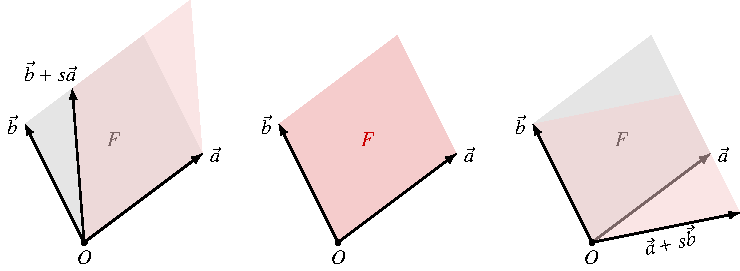
\includegraphics{chapters/040-green/images/parallelogramm.pdf}
\caption{Die Parallelogrammfläche ist eine bilineare Funktion der
Kantenvektoren.
Die Parallelogrammfläche ändert nicht, wenn man einen Kantenvektor
um ein Vielfaches des anderen ändert.
Dies ist die gemeinsame Eigenschaft vieler physikalischer Eigenschaften,
die oft mit dem Vektorprodukt modelliert werden.
\label{buch:green:2vektoren:fig:parallelogramm}}
\end{figure}

Zwei Vektoren $\vec{a}$ und $\vec{b}$ spannen eine Parallelogramm auf.
Der Flächeninhalt ändert sich nicht, wenn man die Spitze des Vektors
$\vec{a}$ parallel zur Richtung von $\vec{b}$ verschiebt.
Er ändert sich auch nicht, wenn man die Spitze von $\vec{b}$ parallel
zur Richtung von $\vec{a}$ verschiebt.

Das Vektorprodukt hat die passenden Eigenschaften.
Ändert man den Vektor $\vec{a}$ in $\vec{a}+t\vec{b}$, ändert sich das
Vektorprodukt
\begin{equation}
(\vec{a}+t\vec{b})\times\vec{b}
=
\vec{a}\times\vec{b} + t(\underbrace{\vec{b}\times\vec{b}}_{\displaystyle=0})
=
\vec{a}\times\vec{b}
\label{buch:green:2vektoren:eqn:parallelogramm1}
\end{equation}
nicht.
Ebenso ändert sich das Vektorprodukt nicht, wenn man $\vec{b}$ durch
$\vec{b}+s\vec{a}$ ersetzt, denn
\begin{equation}
\vec{a}\times(\vec{b}+s\vec{a})
=
\vec{a}\times\vec{b}
+
s(\underbrace{\vec{a}\times\vec{a}}_{\displaystyle=0})
=
\vec{a}\times\vec{b}.
\label{buch:green:2vektoren:eqn:parallelogramm2}
\end{equation}
Für Vektoren im dreidimensionalen Raum ist das Vektorprodukt ein 
Realisierung der einleitend formulierten Eigenschaften.
Die Eigenschaft ist aber auch korrekt in zwei Dimensionen, wo es
das Vektorprodukt nicht gibt.

Der Flächeninhalt eines Parallelogramms ist ausser in zwei Dimensionen
nicht nur eine Zahl, die Lage des Parallelgramms gehört genauso zur
vollständigen Beschreibung der Parallelogrammfläche.
Das Vektorprodukt in drei Dimensionen trägt dem Rechnung, indem
es als Normale auf dem Parallelgramm die Orientierung im dreidimensionalen
Raum festlegt.
In einem höherdimensionalen Raum reicht jedoch ein einzelner auf
einem Parallelogramm orthogonaler Vektor nicht aus, um die Lage im
Raum vollständig festzulegen.

Eine Parallelogrammfläche wird also beschrieben durch ein neues
mathematisches Objekt, welches mit einer bilinearen Operation aus
zwei Vektoren $\vec{a}$ und $\vec{b}$ gebildet wird.
Wir bezeichnen es provisorisch als den 2-Vektor $\vec{a}\wedge\vec{b}$.
Das Zeichen $\wedge$ funktioniert wie ein Produkt, es ist eine 
bilineare Operation zwischen Vektoren mit den Rechenregeln
\begin{align}
(\vec{a}_1+\vec{a}_2)\wedge\vec{b}
&=
\vec{a}_1\wedge\vec{b}+\vec{a}_2\wedge\vec{b}
\notag
\\
\vec{a}\wedge(\vec{b}_1+\vec{b}_2)
&=
\vec{a}\wedge\vec{b}_1 + \vec{a}\wedge\vec{b}_2
\notag
\\
(\lambda\vec{a})\wedge\vec{b}
&=
\lambda(\vec{a}\wedge\vec{b})=\vec{a}\wedge(\lambda\vec{b})
\notag
\\
\vec{a}\wedge\vec{a}&=0.
\label{buch:green:2vektoren:eqn:aa0}
\end{align}
Die ersten drei Regeln drücken aus, dass der 2-Vektor $\vec{a}\wedge\vec{b}$
bilinear ist oder gleichbedeutend, dass das Wedge-Produkt das
Distributivgesetz erfüllt.
Die letzte Regel genügt, um die zu
\eqref{buch:green:2vektoren:eqn:parallelogramm1}
und
\eqref{buch:green:2vektoren:eqn:parallelogramm2}
äquivalenten Regeln
\begin{equation}
\begin{aligned}
\vec{a}\wedge(\vec{b}+t\vec{a})
&=
\vec{a}\wedge\vec{b}
\qquad \forall t\in\mathbb{R}
\\
(\vec{a}+s\vec{b})\wedge\vec{b}
&=
\vec{a}\wedge\vec{b}
\qquad \forall s\in\mathbb{R}
\end{aligned}
\label{buch:green:2vektoren:eqn:grundeigenschaft}
\end{equation}
für das Wedge-Produkt sicherzustellen.
Aus \eqref{buch:green:2vektoren:eqn:aa0} lässt sich aber auch
ableiten, dass für beliebige Vektoren $\vec{a}$ und $\vec{b}$
\begin{align*}
0
&=
(\vec{a}+\vec{b})\wedge(\vec{a}+\vec{b})
\\
&=
\underbrace{\vec{a}\wedge\vec{a}}_{\displaystyle=0}
+
\vec{a}\wedge\vec{b}
+
\vec{b}\wedge\vec{a}
+
\underbrace{\vec{b}\wedge\vec{b}}_{\displaystyle=0}
\\
\Rightarrow\qquad
\vec{a}\wedge\vec{b}
&=
-\vec{b}\wedge\vec{a}
\end{align*}
gilt, das Wedge-Produkt ist also notwendigerweise antikommutativ.

%
% Drehmoment und Drehimpuls
%
\subsubsection{Drehmoment und Drehimpuls}
Eine Kraft $\vec{F}$, die auf einen im Nullpunkt drehbar gelagerten
starren Körper wirkt, versucht diesen Körper in Drehung zu versetzen.
Der Angriffspunkt $P$ der Kraft habe den Ortsvekor $\vec{r}$.
Je grösser die Kraft $\vec{F}$ oder je länger der Vektor $\vec{r}$,
desto grösser wird auch die Drehwirkung sein.
Wir haben also wieder mit einer physikalischen Grösse zu tun, die
bilinear von zwei Vektoren abhängt.

Ändert man die Kraft, indem man eine Komponente parallel zu $\vec{r}$
hinzufügt, dann ändert sich die Auswirkung auf den Drehzustand des
Körpers nicht.
Sie ändert sich auch nicht, wenn man den Ansatzpunkt der Kraft
auf einer Geraden durch den Punkt $P$ mit Richtung $\vec{F}$
verschiebt.
In der Physik wird dies oft dadurch ausgedrückt, dass die Kraft
ein linienflüchtiger Vektor sei.
Diese Eigenschaften decken sich wieder mit den Regeln
\eqref{buch:green:2vektoren:eqn:grundeigenschaft}
des Wedge-Produktes.

In der Physik wird das Drehmoment meistens als Vektorprodukt
$\vec{M}=\vec{r}\times\vec{F}$ modelliert.
Die Überlegungen des vorangegangenen Abschnitts zeigen, dass
es genausogut oder sogar besser durch den 2-Vektor
$\vec{r}\wedge\vec{F}$ beschrieben werden kann.

Beim Drehimpuls wird die Unzulänglichkeit des einfachen, auf
dem Vektorprodukt basierenden Modells offensichtlich.
Versucht man die Drehung durch einen Vektor $\vec{\omega}$ zu
beschreiben, der die Richtung der Drehachse und die Winkelgeschwindigkeit
als Länge enthält, dann ist der Drehimpuls nicht notwendigerweise
parallel zur Richtung der Drehachse.
Vielmehr gibt es eine lineare Abbildung, die den Drehimpulsvektor
$\vec{L}$ aus $\vec{omega}$ berechnet.
Man darf erwarten, dass die Verwirrung aufgelöst wird, wenn man
Drehmoment und Drehimpuls als 2-Vektoren modelliert und den Zusammenhang
dazwischen durch einen Tensor erklärt.

%
% Lorentz-Kraft
%
\subsubsection{Lorentz-Kraft}
%
% fig-lorentz.tex
%
% (c) 2025 Prof Dr Andreas Müller
%
\begin{figure}
\centering
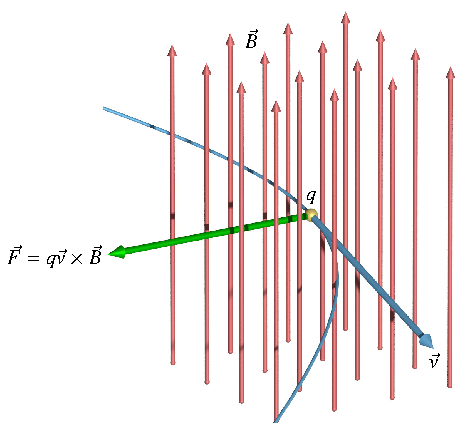
\includegraphics{chapters/040-green/images/lorentz.pdf}
\caption{Die Lorentz-Kraft auf eine bewegte Ladung hängt bilinear
von der Geschwindigkeit $\vec{v}$ und vom magnetischen Induktionsfeld
$\vec{B}$ ab.
Sie hat die Eigenschaften eines 2-Vektors.
\label{buch:green:2vektoren:fig:lorentz}}
\end{figure}

Die Lorentz-Kraft ist die Kraft, die eine bewegte Ladung in einem
magnetischen Feld erfährt.
Sie ist proportional zur Geschwindigkeit, eine ruhende Ladung
wird von einem Magnetfeld nicht beeinflusst.
Sie ist auch proportional zur Stärke des magnetischen Feldes.
Die Lorentz-Kraft ist also eine bilineare Funktion der
Geschwindigkeit $\vec{v}$ der Ladung und des magnetischen
Induktionsfeldes $\vec{B}$

Die Lorentz-Kraft verschwindet, falls sich die Ladung parallel zur
magnetischen Feldrichtung bewegt.
Insbesondere ändert sie auch nicht, wenn die Geschwindigkeit der
Ladung um eine Komponenten parallel zu $\vec{B}$ verändert wird.
Umgekehrt ändert die Lorentz-Kraft auch nicht, wenn dem Feld
eine Komponenten parallel zur Geschwindigkeit der Ladung hinzugefügt
wird.
Auch die Lorentz-Kraft erfüllt also die grundlegenden
Rechenregeln \eqref{buch:green:2vektoren:eqn:grundeigenschaft}.
In der Physik wird sie daher meistens als das Vektorprodukt
\[
\vec{F}_L
=
q\vec{v}\times \vec{B}
\]
beschrieben, worin $q$ die Ladung ist.
Nach den früheren Überlegungen ist sie aber eher als ein weiteres
Beispiel eines 2-Vektors anzusehen.

Es wird sich später zeigen, dass die Elektrodynamik besser in einer
vierdimensionalen Raumzeit beschrieben wird, die auch die Basis für
die spezielle und allgemeine Relatiitätstheorie ist.
Die Identifikation von 2-Vektoren mit Vektoren ist darin nicht
mehr möglich.
Die Verwendung von 2-Vektoren wird aber ermöglichen, die elektrische 
und die Lorentz-Kraft auf einheitliche Art zu beschreiben.

%
% Basis, Wedge-Produkt, Rechenregeln
%
\subsection{Der Vektorraum der 2-Vektoren}
Die 2-Vektoren sind also eine neue Art von Vektoren, die aus den
gewöhnlichen Vektoren in $\mathbb{R}^n$ gebildet werden können.
Sie bilden selbst wieder einen Vektorraum, da man sie addieren
und mit reellen Zahlen multiplizieren kann.
In gewissen Fällen, zum Beispiel im dreidimensionalen Raum, kann
man für 2-Vektoren wieder eine anschauliche Darstellung ähnlich den
Pfeilen für Vektoren finden.
Es wurde aber bereits darauf hingewiesen, dass die eigentlich nicht
zulässig ist, da weder die Dimensionen noch die Symmetrieeigenschaften
vergleichbar sind.
Wenn zwei Vektoren geometrische Längen beschreiben, dann haben sie
die Längeneinheit als Masseinheit.
Ihr Wedge-Produkt muss dann die Flächeneinheit als Masseinheit haben,
kann also nicht im gleichen Raum dargestellt werden.

\subsubsection{Basis}
Ausgehend von der Basis $\vec{e}_1,\dots,\vec{e}_n$ lassen sich jetzt
alle Wedge-Produkte
\[
\vec{e}_i\wedge \vec{e}_k
\]
mit $i\ne k$ bilden.
Wegen
\[
\vec{e}_i\wedge\vec{e}_k
=-
\vec{e}_k\wedge\vec{e}_i
\]
können wir auf die Produkte $\vec{e}_i\wedge\vec{e}_k$ mit $i<k$
beschränken, die wir alle als linear unabhängig annehmen müssen.

\begin{definition}[Raum der 2-Vektoren]
Sei $V$ ein $n$-dimensioinaler reeller Vektorraum, dann ist die Menge
\[
{\textstyle
\bigwedge^2 V}
= \langle \vec{a}\wedge\vec{b} \mid \vec{a},\vec{b}\in V \rangle
\]
ein $n(n-1)/2$-dimensionaler reeller Vektorraum.
Bilden $b_1,\dots,b_n\in V$  eine Basis von $V$, dann bilden die Vektoren
\[
b_i\wedge b_k,\qquad i<k
\]
eine Basis von $\bigwedge^2 V$.
\end{definition}

In einem zweidimensionalen Raum $\mathbb{R}^2$ gibt es nur einen
einzigen 2-Vektor $\vec{e}_1\wedge\vec{e}_2$, nur schon aus diesem
Grund ist es nicht möglich, einen 2-Vektor als Vektor in $\mathbb{R}^2$
darzustellen.

In einem dreidimensionalen Raum $\mathbb{R}^3$ gibt es die drei
Basisvektoren
\[
\vec{e}_1\wedge\vec{e}_2,\quad
\vec{e}_1\wedge\vec{e}_3
\quad\text{und}\quad
\vec{e}_2\wedge\vec{e}_3.
\]
Tatsächlich lässt sich auch eine Abbildung der 2-Vektoren auf
die Vektoren finden, die das Wedge-Produkt auf das Vektorprodukt
abbildet.
Sie wird aus der Komponentenformel weiter unten abgeleitet.

In einem vierdimensionalen Raum $\mathbb{R}^4$ gibt es die sechs
linear unabhängigen Basisvektoren
\[
\vec{e}_1\wedge\vec{e}_2,\quad
\vec{e}_1\wedge\vec{e}_3,\quad
\vec{e}_1\wedge\vec{e}_4,\quad
\vec{e}_2\wedge\vec{e}_3,\quad
\vec{e}_2\wedge\vec{e}_4,
\quad\text{und}\quad
\vec{e}_3\wedge\vec{e}_4.
\]
Da der Raum der 2-Vektoren mehr Dimensionen als der Raum 
der Vektoren hat, ist es grundsätzlich unmöglich, die 2-Vektoren
durch Vektoren zu visualisieren.

\subsubsection{Komponentenformel}
In der Basis $\vec{e}_1,\dots,\vec{e}_n$ kann jeder Vektor als
Linearkombination
\[
\vec{a}
=
a^1\vec{e}_1+\dots+a^n\vec{e}_n
=
\sum_{i=1}^n a^i\vec{e}_i
\qquad\text{und}\qquad
\vec{b}
=
b^1\vec{e}_1+\dots+b^n\vec{e}_n
\sum_{k=1}^n b^k\vec{e}_k
\]
geschrieben werden.
Das Wedge-Produkt der beiden Vektoren ist
\begin{align}
\vec{a}\wedge\vec{b}
&=
\biggl(
\sum_{i=1}^n a^i\vec{e}_i
\biggr)
\wedge
\biggl(
\sum_{k=1}^n b^k\vec{e}_k
\biggr)
\notag
\\
&=
\sum_{i,k=1}^n a^ib^k\,\vec{e}_i\wedge\vec{e}_k
\notag
\intertext{Die Wedge-Produkt $\vec{e}_i\wedge\vec{e}_i=0$ verschwinden,
es bleibt daher nur}
&=
\sum_{i\ne k} a^ib^k \, \vec{e}_i\wedge\vec{e}_k.
\notag
\intertext{Als Basis werden aber nur die Produkte mit $i<k$ verwendet,
wir zerlegen die Summe daher in die Fälle $i<k$ und $k<i$:}
&=
\sum_{i < k} a^ib^k \, \vec{e}_i\wedge\vec{e}_k
+
\sum_{i > k} a^ib^k \, \vec{e}_i\wedge\vec{e}_k
\notag
\\
&=
\sum_{i < k} a^ib^k \, \vec{e}_i\wedge\vec{e}_k
-
\sum_{i > k} a^ib^k \, \vec{e}_k\wedge\vec{e}_i.
\notag
\intertext{In der zweiten Summe ist der erste Index jetzt wieder kleiner
als der zweite, wir können in dieser Summe die Indizes umbennennen
und erhalten}
&=
\sum_{i < k} a^ib^k \, \vec{e}_i\wedge\vec{e}_k
-
\sum_{k > i} a^kb^i \, \vec{e}_i\wedge\vec{e}_k.
\notag
\intertext{Damit können die beiden Summen wieder in eine einzige
zusammengefasst werden.
Daraus lassen sich die Komponenten von}
\vec{a}\wedge\vec{b}
&=
\sum_{i<k} (a^ib^k-a^kb^i)\,\vec{e}_i\wedge\vec{e}_k
\label{buch:green:2vektoren:eqn:komponentenformel}
\end{align}
in der Basis der 2-Vektoren $\vec{e}_i\wedge\vec{e}_k$ ausdrücken.

\subsubsection{Komponentenformel und Vektorprodukt}
Das Vektorprodukt wird in Komponenten als
\[
\begin{pmatrix} a^1 \\ a^2 \\ a^3 \end{pmatrix}
\times
\begin{pmatrix} b^1 \\ b^2 \\ b^3 \end{pmatrix}
=
\begin{pmatrix} a^2b^3-a^3b^2 \\ a^3b^1-a^1b^3 \\ a^1b^2-a^2b^1 \end{pmatrix}
\]
definiert.
Die Komponenten des Vektorprodukts sehen der allgemeinen
Komponentenformel~\eqref{buch:green:2vektoren:eqn:komponentenformel}
des Wedge-Produktes sehr ähnlich.
Tatsächlich kann man den Zusammenhang noch etwas offensichtlicher
machen, indem man die lineare Abbildung $f:\bigwedge^2V\to V$
verwendet, die auf den Basisvektoren durch
\[
\vec{e}_1\wedge\vec{e}_2 \mapsto \vec{e}_3
\vec{e}_1\wedge\vec{e}_3 \mapsto -\vec{e}_2
\vec{e}_2\wedge\vec{e}_3 \mapsto \vec{e}_1
\]
definiert sind.
Aus dem 2-Vektor $\vec{a}\wedge\vec{b}$ wird dadurch
\begin{align*}
f(\vec{a}\wedge\vec{b})
&=
f\bigl((a^1b^2-a^2b^1)\vec{e}_1\wedge\vec{e}_2
      +(a^1b^3-a^3b^1)\vec{e}_1\wedge\vec{e}_3
      +(a^2b^3-a^3b^2)\vec{e}_2\wedge\vec{e}_3\bigr)
\\
&=
(a^1b^2-a^2b^1)\,f(\vec{e}_1\wedge\vec{e}_2)
+(a^1b^3-a^3b^1)\,f(\vec{e}_1\wedge\vec{e}_3)
+(a^2b^3-a^3b^2)\,f(\vec{e}_2\wedge\vec{e}_3)
\\
&=
(a^1b^2-a^2b^1) \vec{e}_3
+(a^1b^3-a^3b^1) (-\vec{e}_2)
+(a^2b^3-a^3b^2) \vec{e}_1
\\
&=
(a^2b^3-a^3b^2) \vec{e}_1
+(a^3b^1-a^1b^3) \vec{e}_2
+(a^1b^2-a^2b^1) \vec{e}_3
\\
&=
\vec{a}\times\vec{b}.
\end{align*}
In diesem Lichte kann man das Vektorprodukt als ein spezielle Darstellung
des Wedge-Produktes durch Vektoren statt 2-Vektoren ansehen, die allerdings
nur in drei Dimensionen möglich ist.

%
% Alternative Darstellungen des Wedge-Produktes
%
\subsection{Alternative Darstellungen des Wedge-Produktes}
Die algebraischen Eigenschaften der 2-Vektoren und des Wedge-Produktes
wurden aus geometrischen oder physikalischen Prinzipien hergeleitet.
Angesichts der Vielfalt der mathematischen Werkzeuge, die zur Beschreibung
der physikalischen Realität zur Verfügung stehen, erwartet man daher,
dass die algebraische Struktur sich in verschiedenen mathematischen
Konstrukten wiederfinden lässt.

\subsubsection{Das Vektorprodukt als Kommutator von Matrizen}
Wir betrachten die Menge 
\[
V
=
\{ A\in M_3(\mathbb{R}) \mid A^t=-A\}
\]
der antisymmetrischen $3\times 3$-Matrizen.
Solche Matrizen sind von der Form
\begin{equation}
A
=
\begin{pmatrix}
  0  &  a_3 & -a_2 \\
-a_3 &   0  &  a_1 \\
 a_2 & -a_1 &   0
\end{pmatrix}.
\label{buch:green:2vektoren:eqn:antisym}
\end{equation}
Der {\em Kommutator} zweier Matrizen ist $[A,B]=AB-BA$ und ergibt
für Matrizen der Form~\eqref{buch:green:2vektoren:eqn:antisym}
\begin{align*}
AB
&=
\begin{pmatrix}
  0  &  a_3 & -a_2 \\
-a_3 &   0  &  a_1 \\
 a_2 & -a_1 &   0
\end{pmatrix}
\begin{pmatrix}
  0  &  b_3 & -b_2 \\
-b_3 &   0  &  b_1 \\
 b_2 & -b_1 &   0
\end{pmatrix}
\\
&=
\begin{pmatrix}
-a_2b_2-a_3b_3 &     a_2b_1     & a_3b_1         \\
 a_1b_2        & a_1b_1+a_3b_3  & a_3b_2         \\
 a_1b_3        &     a_2b_3     & -a_1b_1-a_2b_2 
\end{pmatrix}
\\
BA
&=
\begin{pmatrix}
  0  &  b_3 & -b_2 \\
-b_3 &   0  &  b_1 \\
 b_2 & -b_1 &   0
\end{pmatrix}
\begin{pmatrix}
  0  &  a_3 & -a_2 \\
-a_3 &   0  &  a_1 \\
 a_2 & -a_1 &   0
\end{pmatrix}
\\
&=
\begin{pmatrix}
-a_2b_2-a_3b_3  &      a_1b_2    &    a_1b_3     \\
     a_2b_1     & -a_1b_1-a_3b_3 &    a_2b_3     \\
     a_3b_1     &      a_3b_2    & -a_1b_1-a_2b_2
\end{pmatrix}
\\
[A,B]
&=
AB-BA
=
\begin{pmatrix}
        0        &   a_2b_1-a_1b_2  & -(-a_3b_1+a_1b_3) \\
-(a_2b_1-a_1b_2) &         0        &    a_3b_2-a_2b_3  \\
  a_1b_3-a_3b_1  & -(a_3b_2-a_2b_3) &          0
\end{pmatrix}.
\end{align*}
Diese Matrix ist wieder von der Form 
\eqref{buch:green:2vektoren:eqn:antisym}
und die Einträge sind die Komponenten des Vektorproduktes.
Das Vektorprodukt lässt sich also durch den Matrixkommutator
auf der Menge darstellen.

\subsubsection{Die Lie-Algebra einer Matrizengruppe}
TODO XXX

